\begin{figure*}[t]
\centering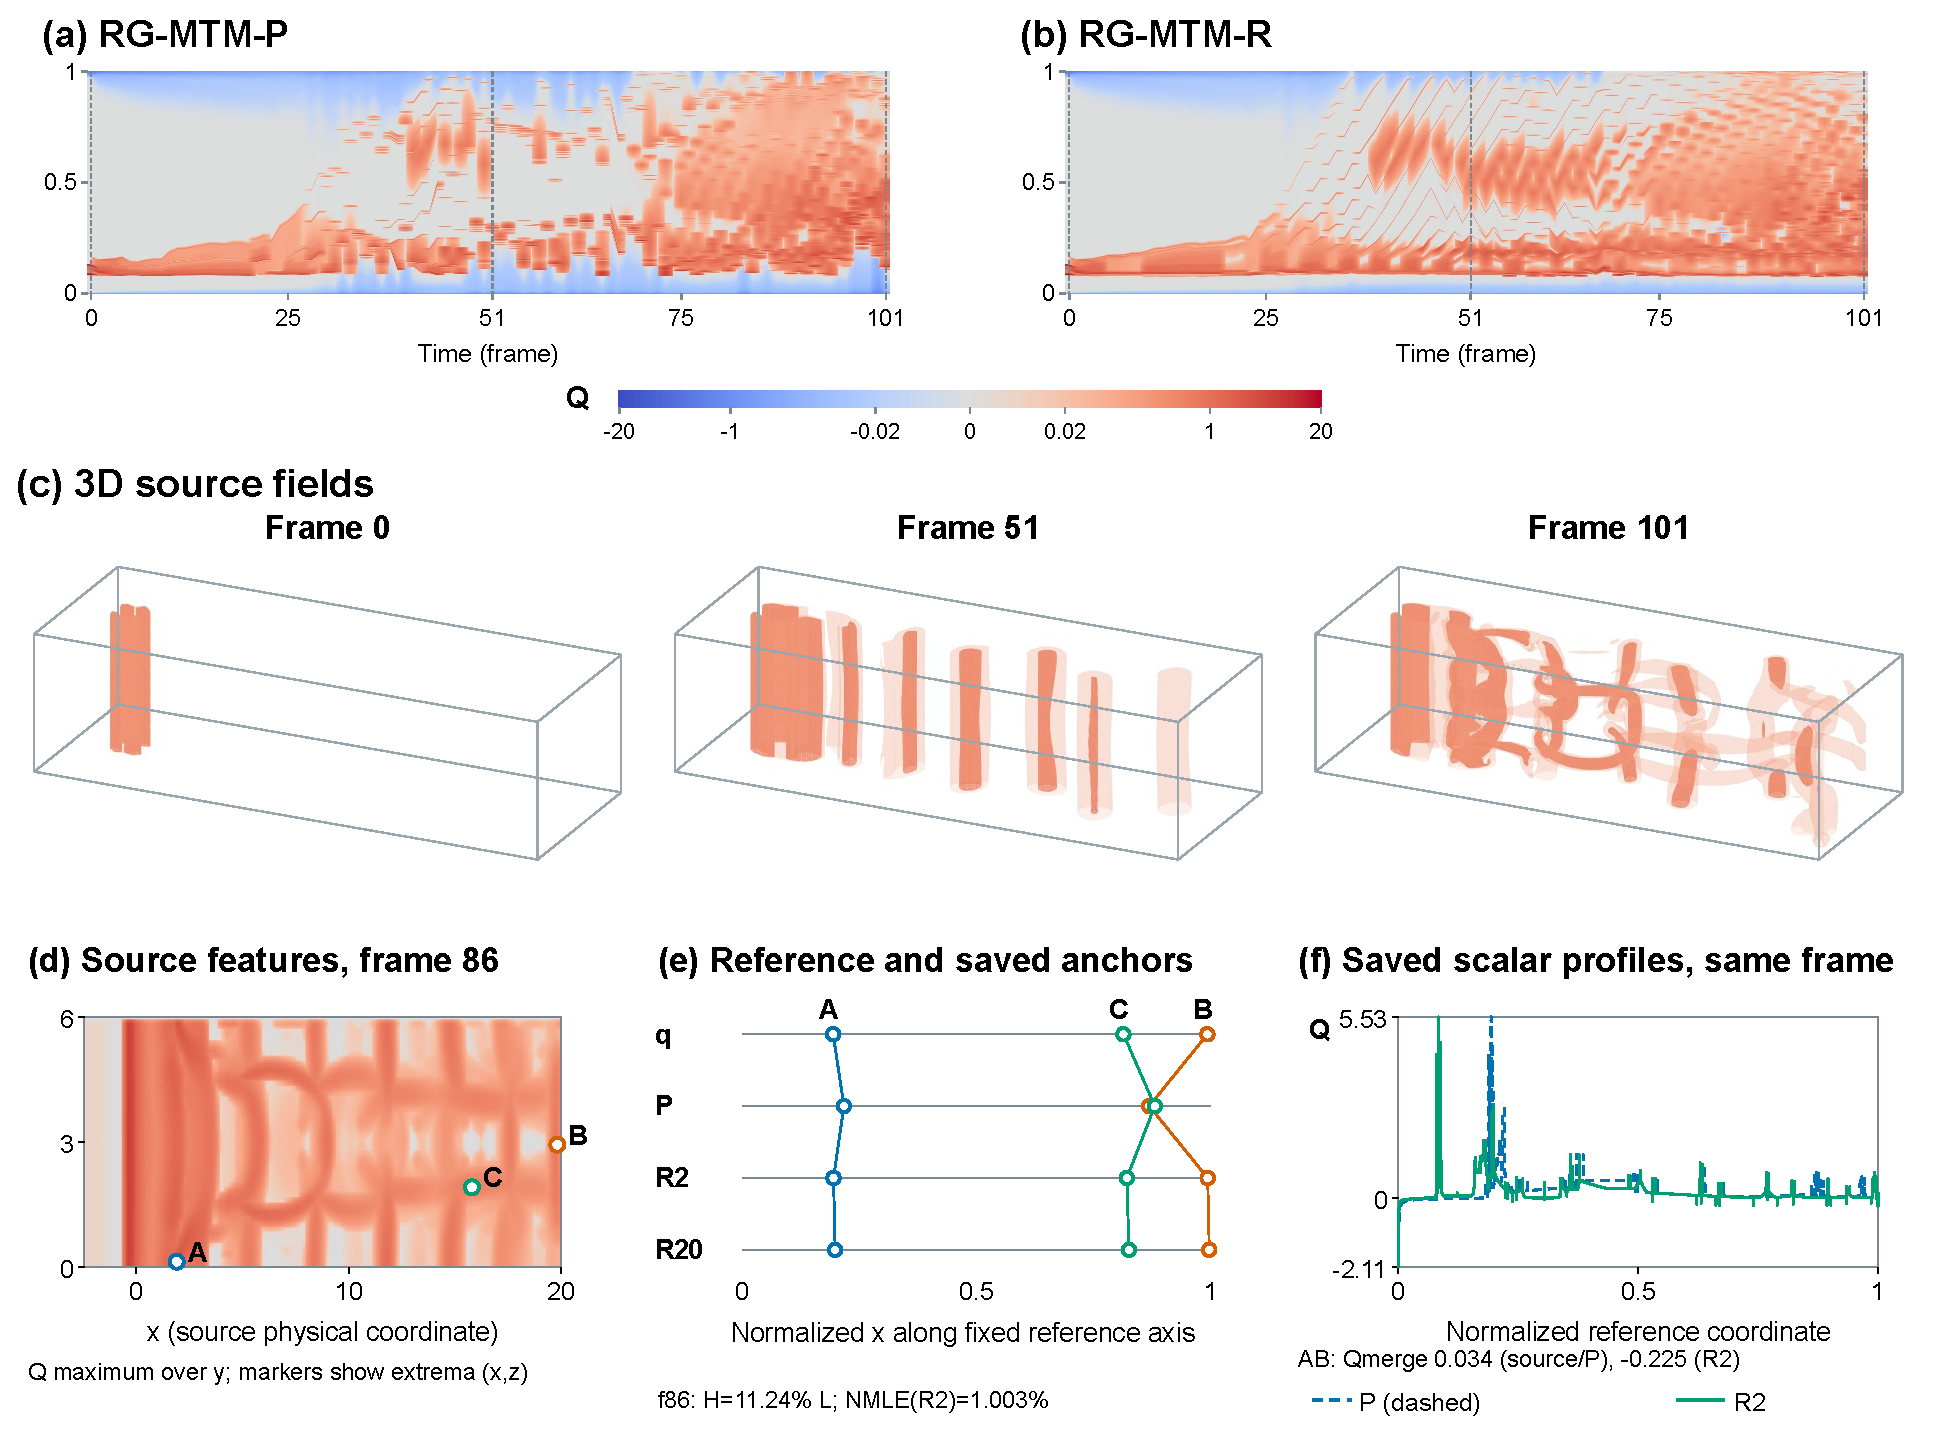
\includegraphics[width=\textwidth]{figures/Fig11.pdf}
\caption{Cylinder: RG-MTM-P (a) and R20 (b) for all 102 original-grid three-dimensional $Q$ fields, with source isosurfaces at frames 0, 51, and 101 (c). The maps use normalized physical $x$ reference position; vertical guides locate the source views. Their common symmetric-log colour scale is linear within $\pm0.02$. Isosurfaces at $Q=0.1$ (translucent) and $0.5$ (solid) share physical aspect, camera, and domain frame. Source views precede persistence simplification; maps use the common simplified inputs. Full TMTM/R2 panels and rendering details are in Supplement S9--S10. Panels (d)--(f) link a median-criterion selected conflict at frame 86 to its source features, continuous anchors and complete P/R2 profiles. Maximum displacement changes from 12.40\% to 1.17\% of reference extent, with 1.003\% R2 NMLE. The local case is descriptive; full-sequence scores remain in the common tables. The source projection in (d) uses bilinear display reconstruction with exact original cell centers. Temporal colour transitions use display interpolation only; saved frames, anchors, and evaluation samples are unchanged.}
\label{fig:cylinder}
\end{figure*}
